\chapter{Analisis}
\label{chap:analysis}

\section{Analisis Aplikasi Sejenis}
\label{sec:analysis-similarapps}

Untuk pembuatan perangkat lunak dalam skripsi ini, ada dua buah perkakas \cl yang akan diamati sebagai aplikasi sejenis, yaitu \chromewebstorecli dan \textit{iTunes Search API}.

\subsection{\chromewebstorecli\footnote{\href{https://github.com/pandawing/node-chrome-web-store-item-property-cli}{https://github.com/pandawing/node-chrome-web-store-item-property-cli}}}
\label{sec:similarapps-chromewebstore}

Perkakas \cl ini merupakan ekstensi dari sebuah aplikasi lain yang memiliki fungsi yang sama, yaitu \textit{Chrome Web Store Item Property}\footnote{\href{https://github.com/pandawing/node-chrome-web-store-item-property}{https://github.com/pandawing/node-chrome-web-store-item-property}}. Perangkat lunak \textit{Chrome Web Store Item Property} ini merupakan perangkat lunak yang akan memanggil fungsi API untuk mendapatkan metadata dari sebuah ekstensi pada \textit{web store} peramban Google Chrome. Perbedaan dari perkakas ini dengan aplikasi dasarnya adalah bahwa perkakas ini dapat digunakan sebagai perkakas \textit{command line}, sedangkan aplikasi dasarnya hanya bisa digunakan dalam perangkat lunak lainnya sebagai pemanggil fungsi API.

\subsubsection{Penggunaan}
\label{sec:similarapps-chromewebstore-usage}

Perkakas ini dapat digunakan melalui \textit{command prompt} dengan cara mengetikkan perintah sebagai berikut.

\begin{verbatim}
                     chrome-web-store-item-property <identifier>
\end{verbatim}

Dengan \verb|identifier| berupa ID dari ekstensi yang diinginkan. Jadi, misalkan pengguna memasukkan \verb|gighmmpiobklfepjocnamgkkbiglidom| sebagai ID yang akan digunakan sebagai \textit{identifier}, maka perkakas ini akan mengembalikan metadata dari ekstensi ``AdBlock'' sebagai keluarannya. Contoh penggunaan perkakas ini dapat dilihat di gambar \ref{fig:similarapps-chromewebstorecli}.

\begin{figure}[ht]
    \centering
    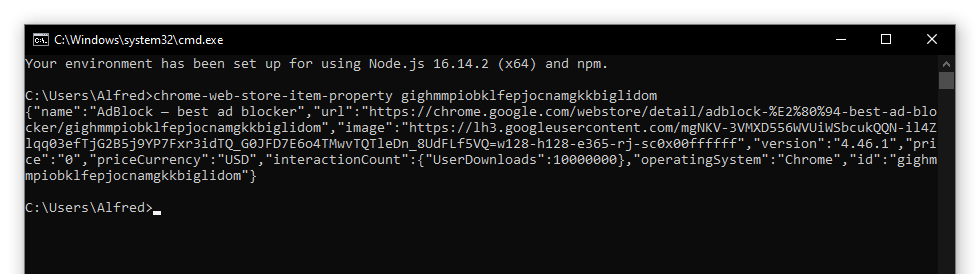
\includegraphics[width=0.75\linewidth]{chromewebstorecli}
    \caption[Contoh penggunaan perkakas \chromewebstorecli]{Contoh penggunaan perkakas \chromewebstorecli.}
    \label{fig:similarapps-chromewebstorecli}
\end{figure}

Sedangkan, keluaran dari perkakas ini merupakan sebuah objek JSON dengan properti-properti sebagai berikut.

\begin{itemize}
	\item \verb|name|\\
	Nama dari ekstensi yang dicari metadatanya.
	\item \verb|url|\\
	URL halaman web dari ekstensi yang dicari di \textit{web store} Google Chrome.
	\item \verb|image|\\
	Logo (dan ikon \textit{thumbnail}) dari ekstensi yang dicari metadatanya.
	\item \verb|version|\\
	Nomor versi dari ekstensi.
	\item \verb|price|\\
	Harga dari ekstensi. Jika ekstensi tidak memiliki harga yang perlu dibayarkan (gratis), properti ini akan bernilai \verb|0|.
	\item \verb|priceCurrency|\\
	Kode mata uang dari harga ekstensi. Jika ekstensi tidak memiliki harga yang perlu dibayarkan, properti ini akan berisi ``\verb|USD|``.
	\item \verb|interactionCount|\\
	Properti ini berisi interaksi-interaksi pengguna yang tercatat sebagai data di halaman \textit{web store} ekstensi. Pada saat pembuatan skripsi ini, properti ini hanya memiliki satu buah subproperti, yaitu \verb|userDownloads|, yang menandakan berapa kali ekstensi ini telah diunduh oleh pengguna di manapun.
	\item \verb|operatingSystems|\\
	Menandakan di peramban mana ekstensi versi ini dapat diinstal. Karena ekstensi-ekstensinya berada di \textit{web store} Chrome,
	\item \verb|ratingValue| (tidak digunakan lagi)\\
	Peringkat yang diberikan oleh para pengguna ekstensi ini. Nilai dari properti ini berupa skala desimal dari 0.00 sampai dengan 5.00. Di versi terbaru dari perkakas ini, properti ini tidak lagi tersedia dalam keluarannya.
	\item \verb|ratingCount| (tidak digunakan lagi)\\
	Jumlah pengguna yang telah menilai/memberi peringkat ke ekstensi ini. Di versi terbaru dari perkakas ini, properti ini tidak lagi tersedia dalam keluarannya.
	\item \verb|id|\\
	Properti ini mengandung ID dari ekstensi tersebut. Nilai dari properti ini akan sama dengan ID yang digunakan sebagai parameter masukan perkakas.
\end{itemize}

\subsection{\itunesapi\footnote{\href{https://github.com/awcross/itunes-search-api}{https://github.com/awcross/itunes-search-api}}}
\label{sec:similarapps-itunesapi}

Perkakas \cl ini berfungsi untuk melakukan pencarian melalui API iTunes, sehingga seakan-akan pengguna langsung melakukan pencarian di iTunes sendiri. Hasil pencarian yang dilakukan termasuk judul lagu, nama artis, ataupun nama album, dan pengguna dapat memilih secara spesifik objek apa yang ingin dicari.

\subsubsection{Penggunaan}
\label{sec:similarapps-chromewebstore-usage}

Perkakas ini dapat digunakan melalui \textit{command prompt} dengan cara mengetikkan perintah sebagai berikut.

\begin{verbatim}
                      itunes-search-api <input> [<options>]
\end{verbatim}

Dengan \verb|input| berupa nama dari objek yang dicari. Perkakas ini juga memiliki opsi yang masing-masing memiliki parameter tersendiri untuk mempersempit hasil pencarian. Adapun opsi-opsi tersebut dapat dilihat di daftar di bawah ini.

\begin{itemize}
	\item \verb|country|\\
	\textbf{Kemungkinan nilai:} Kode negara dua huruf\\
	Opsi ini menerima parameter berupa kode negara asal dari album atau artis yang dicari.
	\item \verb|entity|\\
	\textbf{Kemungkinan nilai:} \verb|song|, \verb|musicArtist|, atau \verb|album|\\
	Menandakan jenis objek/entitas yang ingin dicari. Opsi ini dapat bernilai \verb|song| untuk pencarian berbasis judul lagu, \verb|musicArtist| untuk pencarian nama artis, atau \verb|album| untuk pencarian nama album. Jika opsi ini tidak dipakai, objek apapun yang memiliki kemiripan dengan \verb|input| dalam salah satu dari ketiga properti ini akan muncul dalam hasil pencarian.
	\item \verb|limit|\\
	\textbf{Kemungkinan nilai:} Bilangan bulat positif\footnote{Opsi ini juga menerima bilangan bulat negatif, tetapi menggunakan sebuah bilangan bulat negatif akan menghilangkan pengaruh opsi ini terhadap hasil keluaran.}\\
	Jumlah hasil pencarian maksimal yang ingin ditampilkan dalam keluaran.
\end{itemize}
\vspace{\baselineskip}
Sedangkan, keluaran dari perkakas ini merupakan sebuah objek JSON yang memiliki dua properti utama, yaitu:

\begin{itemize}
	\item \verb|resultCount|\\
	Properti ini berisi bilangan bulat yang menandakan berapa buah objek yang terdapat dalam hasil pencarian.
	\item \verb|results|\\
	\textit{Array} yang berisi kumpulan objek yang terdapat di dalam hasil pencarian. Objek-objek ini akan dikembalikan berupa sebuah \textit{array} lain yang berisi seluruh properti dari masing-masing objek. Apa saja properti yang diikutkan dalam \textit{array} tersebut tergantung tipe dari objek dalam hasil pencarian.
\end{itemize}
\vspace{\baselineskip}
Adapun contoh penggunaan dan hasil keluaran perkakas ini dapat dilihat di gambar \ref{fig:similarapps-itunesapi}.

\begin{figure}[ht]
    \centering
    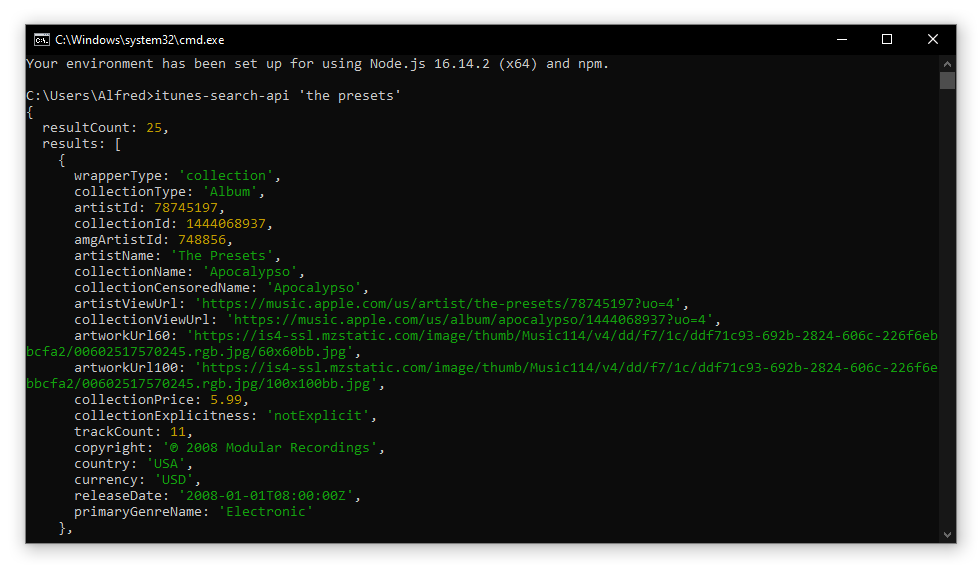
\includegraphics[width=0.75\linewidth]{itunesapi}
    \caption[Contoh penggunaan perkakas \itunesapi]{Contoh penggunaan perkakas \itunesapi.\footnote{Gambar hanya memuat satu objek untuk menghemat tempat.}}
    \label{fig:similarapps-itunesapi}
\end{figure}

\section{Analisis Modul-Modul Bahasa C}
\label{sec:cmodules}



\subsection{getopt}
\label{sec:cmodules-getopt}

